\documentclass[twoside]{book}

% Packages required by doxygen
\usepackage{fixltx2e}
\usepackage{calc}
\usepackage{doxygen}
\usepackage[export]{adjustbox} % also loads graphicx
\usepackage{graphicx}
\usepackage[utf8]{inputenc}
\usepackage{makeidx}
\usepackage{multicol}
\usepackage{multirow}
\PassOptionsToPackage{warn}{textcomp}
\usepackage{textcomp}
\usepackage[nointegrals]{wasysym}
\usepackage[table]{xcolor}

% Font selection
\usepackage[T1]{fontenc}
\usepackage[scaled=.90]{helvet}
\usepackage{courier}
\usepackage{amssymb}
\usepackage{sectsty}
\renewcommand{\familydefault}{\sfdefault}
\allsectionsfont{%
  \fontseries{bc}\selectfont%
  \color{darkgray}%
}
\renewcommand{\DoxyLabelFont}{%
  \fontseries{bc}\selectfont%
  \color{darkgray}%
}
\newcommand{\+}{\discretionary{\mbox{\scriptsize$\hookleftarrow$}}{}{}}

% Page & text layout
\usepackage{geometry}
\geometry{%
  a4paper,%
  top=2.5cm,%
  bottom=2.5cm,%
  left=2.5cm,%
  right=2.5cm%
}
\tolerance=750
\hfuzz=15pt
\hbadness=750
\setlength{\emergencystretch}{15pt}
\setlength{\parindent}{0cm}
\setlength{\parskip}{3ex plus 2ex minus 2ex}
\makeatletter
\renewcommand{\paragraph}{%
  \@startsection{paragraph}{4}{0ex}{-1.0ex}{1.0ex}{%
    \normalfont\normalsize\bfseries\SS@parafont%
  }%
}
\renewcommand{\subparagraph}{%
  \@startsection{subparagraph}{5}{0ex}{-1.0ex}{1.0ex}{%
    \normalfont\normalsize\bfseries\SS@subparafont%
  }%
}
\makeatother

% Headers & footers
\usepackage{fancyhdr}
\pagestyle{fancyplain}
\fancyhead[LE]{\fancyplain{}{\bfseries\thepage}}
\fancyhead[CE]{\fancyplain{}{}}
\fancyhead[RE]{\fancyplain{}{\bfseries\leftmark}}
\fancyhead[LO]{\fancyplain{}{\bfseries\rightmark}}
\fancyhead[CO]{\fancyplain{}{}}
\fancyhead[RO]{\fancyplain{}{\bfseries\thepage}}
\fancyfoot[LE]{\fancyplain{}{}}
\fancyfoot[CE]{\fancyplain{}{}}
\fancyfoot[RE]{\fancyplain{}{\bfseries\scriptsize Generated by Doxygen }}
\fancyfoot[LO]{\fancyplain{}{\bfseries\scriptsize Generated by Doxygen }}
\fancyfoot[CO]{\fancyplain{}{}}
\fancyfoot[RO]{\fancyplain{}{}}
\renewcommand{\footrulewidth}{0.4pt}
\renewcommand{\chaptermark}[1]{%
  \markboth{#1}{}%
}
\renewcommand{\sectionmark}[1]{%
  \markright{\thesection\ #1}%
}

% Indices & bibliography
\usepackage{natbib}
\usepackage[titles]{tocloft}
\setcounter{tocdepth}{3}
\setcounter{secnumdepth}{5}
\makeindex

% Hyperlinks (required, but should be loaded last)
\usepackage{ifpdf}
\ifpdf
  \usepackage[pdftex,pagebackref=true]{hyperref}
\else
  \usepackage[ps2pdf,pagebackref=true]{hyperref}
\fi
\hypersetup{%
  colorlinks=true,%
  linkcolor=blue,%
  citecolor=blue,%
  unicode%
}

% Custom commands
\newcommand{\clearemptydoublepage}{%
  \newpage{\pagestyle{empty}\cleardoublepage}%
}

\usepackage{caption}
\captionsetup{labelsep=space,justification=centering,font={bf},singlelinecheck=off,skip=4pt,position=top}

%===== C O N T E N T S =====

\begin{document}

% Titlepage & ToC
\hypersetup{pageanchor=false,
             bookmarksnumbered=true,
             pdfencoding=unicode
            }
\pagenumbering{alph}
\begin{titlepage}
\vspace*{7cm}
\begin{center}%
{\Large G\+E\+O\+M\+E\+T\+RÍA \\[1ex]\large 0 }\\
\vspace*{1cm}
{\large Generated by Doxygen 1.8.13}\\
\end{center}
\end{titlepage}
\clearemptydoublepage
\pagenumbering{roman}
\tableofcontents
\clearemptydoublepage
\pagenumbering{arabic}
\hypersetup{pageanchor=true}

%--- Begin generated contents ---
\chapter{M\+P1920\+Geometry}
\label{index}\hypertarget{index}{}Given two rectangles and a sequence of points this program calculates which points are inscribed within the intersection of the two rectangles
\begin{DoxyItemize}
\item programmatically sets the data of the first rectangle
\item reads the second rectangle from keyboard
\item calculates the intersection
\begin{DoxyItemize}
\item if the intersection is empty, it ends
\item otherwise it reads the points and for each point
\begin{DoxyItemize}
\item Check if the point belongs the intersection
\item Counts the number of points inscribed in the intersection
\item The sequence ends when a point with any negative coordinate is read 
\end{DoxyItemize}
\end{DoxyItemize}
\end{DoxyItemize}
\chapter{Class Index}
\section{Class List}
Here are the classes, structs, unions and interfaces with brief descriptions\+:\begin{DoxyCompactList}
\item\contentsline{section}{\hyperlink{classPoint2D}{Point2D} \\*To represent a point in a two-\/dimensional space }{\pageref{classPoint2D}}{}
\item\contentsline{section}{\hyperlink{classRectangle}{Rectangle} \\*To represent a rectangle in a two-\/dimensional space as a pair or points, the top-\/left corner and the bottom-\/right one }{\pageref{classRectangle}}{}
\end{DoxyCompactList}

\chapter{File Index}
\section{File List}
Here is a list of all documented files with brief descriptions\+:\begin{DoxyCompactList}
\item\contentsline{section}{src/\hyperlink{main_8cpp}{main.\+cpp} }{\pageref{main_8cpp}}{}
\end{DoxyCompactList}

\chapter{Class Documentation}
\hypertarget{classPoint2D}{}\section{Point2D Class Reference}
\label{classPoint2D}\index{Point2D@{Point2D}}


To represent a point in a two-\/dimensional space.  


\subsection*{Public Member Functions}
\begin{DoxyCompactItemize}
\item 
\mbox{\Hypertarget{classPoint2D_a2415006d697f1c222c17254bdd302098}\label{classPoint2D_a2415006d697f1c222c17254bdd302098}} 
\hyperlink{classPoint2D_a2415006d697f1c222c17254bdd302098}{Point2D} ()
\begin{DoxyCompactList}\small\item\em Basic constructor. \end{DoxyCompactList}\item 
\hyperlink{classPoint2D_a925d8fbd28c1bec7ff05f24c9ce8d182}{Point2D} (int x, int y)
\begin{DoxyCompactList}\small\item\em Constructor with initialization parameters. \end{DoxyCompactList}\item 
void \hyperlink{classPoint2D_af268842e8f2e6072ffe345dc2f322046}{setX} (int px)
\begin{DoxyCompactList}\small\item\em Initializes the X coordinate. \end{DoxyCompactList}\item 
void \hyperlink{classPoint2D_a0e08240b54e6eaae92c979082da1c91c}{setY} (int py)
\begin{DoxyCompactList}\small\item\em Initializes the Y coordinate. \end{DoxyCompactList}\item 
int \hyperlink{classPoint2D_a5cb1c2584e5b2bada0226a3e32aa2b1a}{getX} () const
\begin{DoxyCompactList}\small\item\em Queries the X coordinate. \end{DoxyCompactList}\item 
int \hyperlink{classPoint2D_a53d10f2e460c47a493a3fbadfbafbb64}{getY} () const
\begin{DoxyCompactList}\small\item\em Queries the Y coordinate. \end{DoxyCompactList}\item 
\mbox{\Hypertarget{classPoint2D_ac13d12003e2da9afee19a6a3f526c660}\label{classPoint2D_ac13d12003e2da9afee19a6a3f526c660}} 
void \hyperlink{classPoint2D_ac13d12003e2da9afee19a6a3f526c660}{read} ()
\begin{DoxyCompactList}\small\item\em Reads the XY value from keyboard. \end{DoxyCompactList}\item 
\mbox{\Hypertarget{classPoint2D_a4be0cc5bb62eef12bfa55ced97d03535}\label{classPoint2D_a4be0cc5bb62eef12bfa55ced97d03535}} 
void \hyperlink{classPoint2D_a4be0cc5bb62eef12bfa55ced97d03535}{print} () const
\begin{DoxyCompactList}\small\item\em Prints the XY values in the screen in the form (X,Y) \end{DoxyCompactList}\end{DoxyCompactItemize}


\subsection{Detailed Description}
To represent a point in a two-\/dimensional space. 

Definition at line 31 of file main.\+cpp.



\subsection{Constructor \& Destructor Documentation}
\mbox{\Hypertarget{classPoint2D_a925d8fbd28c1bec7ff05f24c9ce8d182}\label{classPoint2D_a925d8fbd28c1bec7ff05f24c9ce8d182}} 
\index{Point2D@{Point2D}!Point2D@{Point2D}}
\index{Point2D@{Point2D}!Point2D@{Point2D}}
\subsubsection{\texorpdfstring{Point2\+D()}{Point2D()}}
{\footnotesize\ttfamily Point2\+D\+::\+Point2D (\begin{DoxyParamCaption}\item[{int}]{x,  }\item[{int}]{y }\end{DoxyParamCaption})\hspace{0.3cm}{\ttfamily [inline]}}



Constructor with initialization parameters. 


\begin{DoxyParams}{Parameters}
{\em x} & Coordinate \\
\hline
{\em y} & Coordinate \\
\hline
\end{DoxyParams}


Definition at line 46 of file main.\+cpp.


\begin{DoxyCode}
46                           \{
47         px = x;
48         py = y;
49     \}
\end{DoxyCode}


\subsection{Member Function Documentation}
\mbox{\Hypertarget{classPoint2D_a5cb1c2584e5b2bada0226a3e32aa2b1a}\label{classPoint2D_a5cb1c2584e5b2bada0226a3e32aa2b1a}} 
\index{Point2D@{Point2D}!getX@{getX}}
\index{getX@{getX}!Point2D@{Point2D}}
\subsubsection{\texorpdfstring{get\+X()}{getX()}}
{\footnotesize\ttfamily int Point2\+D\+::getX (\begin{DoxyParamCaption}{ }\end{DoxyParamCaption}) const\hspace{0.3cm}{\ttfamily [inline]}}



Queries the X coordinate. 

\begin{DoxyReturn}{Returns}
Value of X 
\end{DoxyReturn}


Definition at line 68 of file main.\+cpp.


\begin{DoxyCode}
68                      \{
69         \textcolor{keywordflow}{return} px;
70     \}
\end{DoxyCode}
\mbox{\Hypertarget{classPoint2D_a53d10f2e460c47a493a3fbadfbafbb64}\label{classPoint2D_a53d10f2e460c47a493a3fbadfbafbb64}} 
\index{Point2D@{Point2D}!getY@{getY}}
\index{getY@{getY}!Point2D@{Point2D}}
\subsubsection{\texorpdfstring{get\+Y()}{getY()}}
{\footnotesize\ttfamily int Point2\+D\+::getY (\begin{DoxyParamCaption}{ }\end{DoxyParamCaption}) const\hspace{0.3cm}{\ttfamily [inline]}}



Queries the Y coordinate. 

\begin{DoxyReturn}{Returns}
Value of Y 
\end{DoxyReturn}


Definition at line 75 of file main.\+cpp.


\begin{DoxyCode}
75                      \{
76         \textcolor{keywordflow}{return} py;
77     \}
\end{DoxyCode}
\mbox{\Hypertarget{classPoint2D_af268842e8f2e6072ffe345dc2f322046}\label{classPoint2D_af268842e8f2e6072ffe345dc2f322046}} 
\index{Point2D@{Point2D}!setX@{setX}}
\index{setX@{setX}!Point2D@{Point2D}}
\subsubsection{\texorpdfstring{set\+X()}{setX()}}
{\footnotesize\ttfamily void Point2\+D\+::setX (\begin{DoxyParamCaption}\item[{int}]{px }\end{DoxyParamCaption})\hspace{0.3cm}{\ttfamily [inline]}}



Initializes the X coordinate. 


\begin{DoxyParams}{Parameters}
{\em px} & New value for X \\
\hline
\end{DoxyParams}


Definition at line 54 of file main.\+cpp.


\begin{DoxyCode}
54                       \{
55         this->px = px;
56     \}
\end{DoxyCode}
\mbox{\Hypertarget{classPoint2D_a0e08240b54e6eaae92c979082da1c91c}\label{classPoint2D_a0e08240b54e6eaae92c979082da1c91c}} 
\index{Point2D@{Point2D}!setY@{setY}}
\index{setY@{setY}!Point2D@{Point2D}}
\subsubsection{\texorpdfstring{set\+Y()}{setY()}}
{\footnotesize\ttfamily void Point2\+D\+::setY (\begin{DoxyParamCaption}\item[{int}]{py }\end{DoxyParamCaption})\hspace{0.3cm}{\ttfamily [inline]}}



Initializes the Y coordinate. 


\begin{DoxyParams}{Parameters}
{\em py} & New value for Y \\
\hline
\end{DoxyParams}


Definition at line 61 of file main.\+cpp.


\begin{DoxyCode}
61                       \{
62         this->py = py;
63     \}
\end{DoxyCode}


The documentation for this class was generated from the following file\+:\begin{DoxyCompactItemize}
\item 
src/\hyperlink{main_8cpp}{main.\+cpp}\end{DoxyCompactItemize}

\hypertarget{classRectangle}{}\section{Rectangle Class Reference}
\label{classRectangle}\index{Rectangle@{Rectangle}}


To represent a rectangle in a two-\/dimensional space as a pair or points, the top-\/left corner and the bottom-\/right one.  


\subsection*{Public Member Functions}
\begin{DoxyCompactItemize}
\item 
\mbox{\Hypertarget{classRectangle_a8a933e0ebd9e80ce91e61ffe87fd577e}\label{classRectangle_a8a933e0ebd9e80ce91e61ffe87fd577e}} 
\hyperlink{classRectangle_a8a933e0ebd9e80ce91e61ffe87fd577e}{Rectangle} ()
\begin{DoxyCompactList}\small\item\em Basic constructor. \end{DoxyCompactList}\item 
\hyperlink{classRectangle_a1546993e9fc10b8d128f4a85ed68c653}{Rectangle} (int x, int y, int w, int h)
\begin{DoxyCompactList}\small\item\em Constructor with parameters. \end{DoxyCompactList}\item 
void \hyperlink{classRectangle_a31c4b9fc0d1ddf912f114da494e50205}{set\+Geometry} (int x, int y, int w, int h)
\begin{DoxyCompactList}\small\item\em Initializes the data of the rectangle. \end{DoxyCompactList}\item 
void \hyperlink{classRectangle_af8d143717fa47878690b12705a687b38}{set\+Geometry} (const \hyperlink{classPoint2D}{Point2D} \&tl, const \hyperlink{classPoint2D}{Point2D} \&br)
\begin{DoxyCompactList}\small\item\em Initializes the data of the rectangle. \end{DoxyCompactList}\item 
\hyperlink{classPoint2D}{Point2D} \hyperlink{classRectangle_a812afd6deed0cdec0b4ad7b2bd93871d}{get\+Top\+Left} () const
\begin{DoxyCompactList}\small\item\em Queries the top-\/left corner. \end{DoxyCompactList}\item 
\hyperlink{classPoint2D}{Point2D} \hyperlink{classRectangle_a5f30a92f3fc197dda50d9e59995d3ac1}{get\+Bottom\+Right} () const
\begin{DoxyCompactList}\small\item\em Queries the bottom-\/right corner. \end{DoxyCompactList}\item 
bool \hyperlink{classRectangle_af732bce8c96d2469994825e9a87dbe5f}{is\+Empty} () const
\begin{DoxyCompactList}\small\item\em For a rectangle to be valid this condition must hold topleft.\+get\+X() $<$ = bottomright.\+get\+X() \&\& topleft.\+get\+Y() $>$ = bottomright.\+get\+Y() otherwise it is an empty (incorrect) rectangle. \end{DoxyCompactList}\item 
\mbox{\Hypertarget{classRectangle_af6973ed3094f9dbabeadb071772fa76d}\label{classRectangle_af6973ed3094f9dbabeadb071772fa76d}} 
void \hyperlink{classRectangle_af6973ed3094f9dbabeadb071772fa76d}{read} ()
\begin{DoxyCompactList}\small\item\em Reads the two points of the rectangle. \end{DoxyCompactList}\item 
\mbox{\Hypertarget{classRectangle_a4e315c59754599c74e99e8b31f7031a0}\label{classRectangle_a4e315c59754599c74e99e8b31f7031a0}} 
void \hyperlink{classRectangle_a4e315c59754599c74e99e8b31f7031a0}{print} () const
\begin{DoxyCompactList}\small\item\em Prints the rectangle in the form \mbox{[}\hyperlink{classPoint2D}{Point2D} -\/ \hyperlink{classPoint2D}{Point2D}\mbox{]}. \end{DoxyCompactList}\end{DoxyCompactItemize}
\subsection*{Friends}
\begin{DoxyCompactItemize}
\item 
\hyperlink{classRectangle}{Rectangle} \hyperlink{classRectangle_a888d2b0113947b4461107bb02b28799d}{do\+Overlap} (const \hyperlink{classRectangle}{Rectangle} \&r1, const \hyperlink{classRectangle}{Rectangle} \&r2)
\begin{DoxyCompactList}\small\item\em Calculates the rectangle intersection of the two given rectangles. If there is no intersection, an empty rectangle is returned instead. \end{DoxyCompactList}\end{DoxyCompactItemize}


\subsection{Detailed Description}
To represent a rectangle in a two-\/dimensional space as a pair or points, the top-\/left corner and the bottom-\/right one. 

Definition at line 97 of file main.\+cpp.



\subsection{Constructor \& Destructor Documentation}
\mbox{\Hypertarget{classRectangle_a1546993e9fc10b8d128f4a85ed68c653}\label{classRectangle_a1546993e9fc10b8d128f4a85ed68c653}} 
\index{Rectangle@{Rectangle}!Rectangle@{Rectangle}}
\index{Rectangle@{Rectangle}!Rectangle@{Rectangle}}
\subsubsection{\texorpdfstring{Rectangle()}{Rectangle()}}
{\footnotesize\ttfamily Rectangle\+::\+Rectangle (\begin{DoxyParamCaption}\item[{int}]{x,  }\item[{int}]{y,  }\item[{int}]{w,  }\item[{int}]{h }\end{DoxyParamCaption})\hspace{0.3cm}{\ttfamily [inline]}}



Constructor with parameters. 


\begin{DoxyParams}{Parameters}
{\em x} & XY Coordinates of top-\/left corner \\
\hline
{\em y} & \\
\hline
{\em w} & Width of the rectangle \\
\hline
{\em h} & Height of the rectangle \\
\hline
\end{DoxyParams}


Definition at line 113 of file main.\+cpp.


\begin{DoxyCode}
113                                           \{
114         topleft.\hyperlink{classPoint2D_af268842e8f2e6072ffe345dc2f322046}{setX}(x);
115         topleft.\hyperlink{classPoint2D_a0e08240b54e6eaae92c979082da1c91c}{setY}(y);
116         bottomright.\hyperlink{classPoint2D_af268842e8f2e6072ffe345dc2f322046}{setX}(x+w-1);
117         bottomright.\hyperlink{classPoint2D_a0e08240b54e6eaae92c979082da1c91c}{setY}(y+h-1);
118         \textcolor{comment}{// setGeometry(x,y,w,h);}
119     \}
\end{DoxyCode}
Here is the call graph for this function\+:
\nopagebreak
\begin{figure}[H]
\begin{center}
\leavevmode
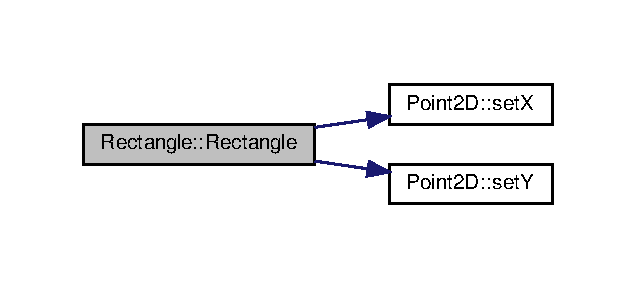
\includegraphics[width=305pt]{classRectangle_a1546993e9fc10b8d128f4a85ed68c653_cgraph}
\end{center}
\end{figure}


\subsection{Member Function Documentation}
\mbox{\Hypertarget{classRectangle_a5f30a92f3fc197dda50d9e59995d3ac1}\label{classRectangle_a5f30a92f3fc197dda50d9e59995d3ac1}} 
\index{Rectangle@{Rectangle}!get\+Bottom\+Right@{get\+Bottom\+Right}}
\index{get\+Bottom\+Right@{get\+Bottom\+Right}!Rectangle@{Rectangle}}
\subsubsection{\texorpdfstring{get\+Bottom\+Right()}{getBottomRight()}}
{\footnotesize\ttfamily \hyperlink{classPoint2D}{Point2D} Rectangle\+::get\+Bottom\+Right (\begin{DoxyParamCaption}{ }\end{DoxyParamCaption}) const\hspace{0.3cm}{\ttfamily [inline]}}



Queries the bottom-\/right corner. 

\begin{DoxyReturn}{Returns}
The point 
\end{DoxyReturn}


Definition at line 154 of file main.\+cpp.


\begin{DoxyCode}
154                                    \{
155         \textcolor{keywordflow}{return} bottomright;
156     \}
\end{DoxyCode}
\mbox{\Hypertarget{classRectangle_a812afd6deed0cdec0b4ad7b2bd93871d}\label{classRectangle_a812afd6deed0cdec0b4ad7b2bd93871d}} 
\index{Rectangle@{Rectangle}!get\+Top\+Left@{get\+Top\+Left}}
\index{get\+Top\+Left@{get\+Top\+Left}!Rectangle@{Rectangle}}
\subsubsection{\texorpdfstring{get\+Top\+Left()}{getTopLeft()}}
{\footnotesize\ttfamily \hyperlink{classPoint2D}{Point2D} Rectangle\+::get\+Top\+Left (\begin{DoxyParamCaption}{ }\end{DoxyParamCaption}) const\hspace{0.3cm}{\ttfamily [inline]}}



Queries the top-\/left corner. 

\begin{DoxyReturn}{Returns}
The point 
\end{DoxyReturn}


Definition at line 147 of file main.\+cpp.


\begin{DoxyCode}
147                                \{
148         \textcolor{keywordflow}{return} topleft;
149     \}
\end{DoxyCode}
\mbox{\Hypertarget{classRectangle_af732bce8c96d2469994825e9a87dbe5f}\label{classRectangle_af732bce8c96d2469994825e9a87dbe5f}} 
\index{Rectangle@{Rectangle}!is\+Empty@{is\+Empty}}
\index{is\+Empty@{is\+Empty}!Rectangle@{Rectangle}}
\subsubsection{\texorpdfstring{is\+Empty()}{isEmpty()}}
{\footnotesize\ttfamily bool Rectangle\+::is\+Empty (\begin{DoxyParamCaption}{ }\end{DoxyParamCaption}) const\hspace{0.3cm}{\ttfamily [inline]}}



For a rectangle to be valid this condition must hold topleft.\+get\+X() $<$ = bottomright.\+get\+X() \&\& topleft.\+get\+Y() $>$ = bottomright.\+get\+Y() otherwise it is an empty (incorrect) rectangle. 

\begin{DoxyReturn}{Returns}
Whether the rectangle is empty or not 
\end{DoxyReturn}


Definition at line 163 of file main.\+cpp.


\begin{DoxyCode}
163                          \{
164         \textcolor{keywordflow}{return} topleft.\hyperlink{classPoint2D_a5cb1c2584e5b2bada0226a3e32aa2b1a}{getX}()>bottomright.\hyperlink{classPoint2D_a5cb1c2584e5b2bada0226a3e32aa2b1a}{getX}() || topleft.\hyperlink{classPoint2D_a53d10f2e460c47a493a3fbadfbafbb64}{getY}() < bottomright.
      \hyperlink{classPoint2D_a53d10f2e460c47a493a3fbadfbafbb64}{getY}();
165     \}
\end{DoxyCode}
Here is the call graph for this function\+:
\nopagebreak
\begin{figure}[H]
\begin{center}
\leavevmode
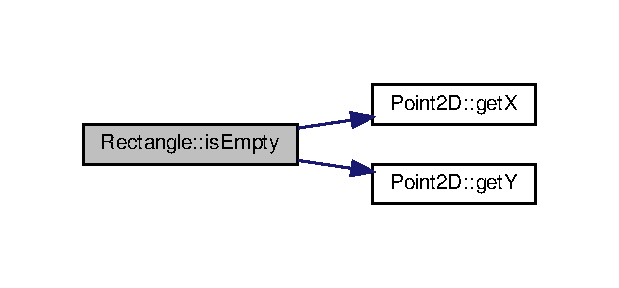
\includegraphics[width=297pt]{classRectangle_af732bce8c96d2469994825e9a87dbe5f_cgraph}
\end{center}
\end{figure}
\mbox{\Hypertarget{classRectangle_a31c4b9fc0d1ddf912f114da494e50205}\label{classRectangle_a31c4b9fc0d1ddf912f114da494e50205}} 
\index{Rectangle@{Rectangle}!set\+Geometry@{set\+Geometry}}
\index{set\+Geometry@{set\+Geometry}!Rectangle@{Rectangle}}
\subsubsection{\texorpdfstring{set\+Geometry()}{setGeometry()}\hspace{0.1cm}{\footnotesize\ttfamily [1/2]}}
{\footnotesize\ttfamily void Rectangle\+::set\+Geometry (\begin{DoxyParamCaption}\item[{int}]{x,  }\item[{int}]{y,  }\item[{int}]{w,  }\item[{int}]{h }\end{DoxyParamCaption})\hspace{0.3cm}{\ttfamily [inline]}}



Initializes the data of the rectangle. 


\begin{DoxyParams}{Parameters}
{\em x} & XY Coordinates of top-\/left corner \\
\hline
{\em y} & \\
\hline
{\em w} & Width of the rectangle \\
\hline
{\em h} & Height of the rectangle \\
\hline
\end{DoxyParams}


Definition at line 128 of file main.\+cpp.


\begin{DoxyCode}
128                                                  \{
129         topleft.\hyperlink{classPoint2D_af268842e8f2e6072ffe345dc2f322046}{setX}(x);
130         topleft.\hyperlink{classPoint2D_a0e08240b54e6eaae92c979082da1c91c}{setY}(y);
131         bottomright.\hyperlink{classPoint2D_af268842e8f2e6072ffe345dc2f322046}{setX}(x+w);
132         bottomright.\hyperlink{classPoint2D_a0e08240b54e6eaae92c979082da1c91c}{setY}(y-h);
133     \}
\end{DoxyCode}
Here is the call graph for this function\+:
\nopagebreak
\begin{figure}[H]
\begin{center}
\leavevmode
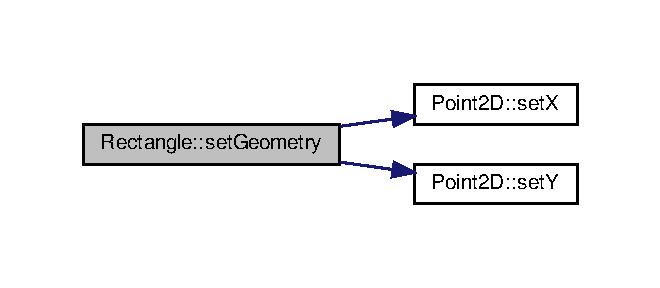
\includegraphics[width=317pt]{classRectangle_a31c4b9fc0d1ddf912f114da494e50205_cgraph}
\end{center}
\end{figure}
\mbox{\Hypertarget{classRectangle_af8d143717fa47878690b12705a687b38}\label{classRectangle_af8d143717fa47878690b12705a687b38}} 
\index{Rectangle@{Rectangle}!set\+Geometry@{set\+Geometry}}
\index{set\+Geometry@{set\+Geometry}!Rectangle@{Rectangle}}
\subsubsection{\texorpdfstring{set\+Geometry()}{setGeometry()}\hspace{0.1cm}{\footnotesize\ttfamily [2/2]}}
{\footnotesize\ttfamily void Rectangle\+::set\+Geometry (\begin{DoxyParamCaption}\item[{const \hyperlink{classPoint2D}{Point2D} \&}]{tl,  }\item[{const \hyperlink{classPoint2D}{Point2D} \&}]{br }\end{DoxyParamCaption})\hspace{0.3cm}{\ttfamily [inline]}}



Initializes the data of the rectangle. 


\begin{DoxyParams}{Parameters}
{\em tl} & Top-\/left point \\
\hline
{\em br} & Bottom-\/right corner \\
\hline
\end{DoxyParams}


Definition at line 139 of file main.\+cpp.


\begin{DoxyCode}
139                                                            \{
140         topleft = tl;
141         bottomright = br;
142     \}
\end{DoxyCode}


\subsection{Friends And Related Function Documentation}
\mbox{\Hypertarget{classRectangle_a888d2b0113947b4461107bb02b28799d}\label{classRectangle_a888d2b0113947b4461107bb02b28799d}} 
\index{Rectangle@{Rectangle}!do\+Overlap@{do\+Overlap}}
\index{do\+Overlap@{do\+Overlap}!Rectangle@{Rectangle}}
\subsubsection{\texorpdfstring{do\+Overlap}{doOverlap}}
{\footnotesize\ttfamily \hyperlink{classRectangle}{Rectangle} do\+Overlap (\begin{DoxyParamCaption}\item[{const \hyperlink{classRectangle}{Rectangle} \&}]{r1,  }\item[{const \hyperlink{classRectangle}{Rectangle} \&}]{r2 }\end{DoxyParamCaption})\hspace{0.3cm}{\ttfamily [friend]}}



Calculates the rectangle intersection of the two given rectangles. If there is no intersection, an empty rectangle is returned instead. 


\begin{DoxyParams}{Parameters}
{\em r1} & One rectangle \\
\hline
{\em r2} & Other rectangle \\
\hline
\end{DoxyParams}
\begin{DoxyReturn}{Returns}
The rectangle given by the intersection of {\ttfamily r1} and {\ttfamily r2} 
\end{DoxyReturn}
\begin{DoxyNote}{Note}
This is an external function to the class \hyperlink{classRectangle}{Rectangle} but since it is also friend, this function is allowed access to private data/methods 
\end{DoxyNote}


Definition at line 198 of file main.\+cpp.


\begin{DoxyCode}
198                                                                \{
199     \hyperlink{classRectangle}{Rectangle} result;
200     \hyperlink{classPoint2D}{Point2D} rTL, rBR;
201     \textcolor{comment}{/* NO FRIEND}
202 \textcolor{comment}{        rTL.setX(max(r1.getTopLeft().getX(),r2.getTopLeft().getX()));}
203 \textcolor{comment}{        rTL.setY(max(r1.getTopLeft().getY(),r2.getTopLeft().getY()));}
204 \textcolor{comment}{        rBR.setX(min(r1.getBottomRight().getX(),r2.getBottomRight().getX()));}
205 \textcolor{comment}{        rBR.setY(min(r1.getBottomRight().getY(),r2.getBottomRight().getY()));}
206 \textcolor{comment}{     */}
207     rTL.\hyperlink{classPoint2D_af268842e8f2e6072ffe345dc2f322046}{setX}(max(r1.topleft.\hyperlink{classPoint2D_a5cb1c2584e5b2bada0226a3e32aa2b1a}{getX}(),r2.topleft.\hyperlink{classPoint2D_a5cb1c2584e5b2bada0226a3e32aa2b1a}{getX}()));
208     rTL.\hyperlink{classPoint2D_a0e08240b54e6eaae92c979082da1c91c}{setY}(min(r1.topleft.\hyperlink{classPoint2D_a53d10f2e460c47a493a3fbadfbafbb64}{getY}(),r2.topleft.\hyperlink{classPoint2D_a53d10f2e460c47a493a3fbadfbafbb64}{getY}()));
209     rBR.\hyperlink{classPoint2D_af268842e8f2e6072ffe345dc2f322046}{setX}(min(r1.bottomright.\hyperlink{classPoint2D_a5cb1c2584e5b2bada0226a3e32aa2b1a}{getX}(),r2.bottomright.\hyperlink{classPoint2D_a5cb1c2584e5b2bada0226a3e32aa2b1a}{getX}()));
210     rBR.\hyperlink{classPoint2D_a0e08240b54e6eaae92c979082da1c91c}{setY}(max(r1.bottomright.\hyperlink{classPoint2D_a53d10f2e460c47a493a3fbadfbafbb64}{getY}(),r2.bottomright.\hyperlink{classPoint2D_a53d10f2e460c47a493a3fbadfbafbb64}{getY}()));
211     result.\hyperlink{classRectangle_a31c4b9fc0d1ddf912f114da494e50205}{setGeometry}(rTL,rBR);
212     \textcolor{keywordflow}{return} result; \textcolor{comment}{// Read more}
213 \}
\end{DoxyCode}


The documentation for this class was generated from the following file\+:\begin{DoxyCompactItemize}
\item 
src/\hyperlink{main_8cpp}{main.\+cpp}\end{DoxyCompactItemize}

\chapter{File Documentation}
\hypertarget{main_8cpp}{}\section{src/main.cpp File Reference}
\label{main_8cpp}\index{src/main.\+cpp@{src/main.\+cpp}}
{\ttfamily \#include $<$iostream$>$}\newline
{\ttfamily \#include $<$cmath$>$}\newline
Include dependency graph for main.\+cpp\+:
\nopagebreak
\begin{figure}[H]
\begin{center}
\leavevmode
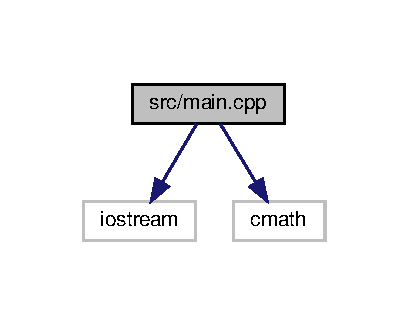
\includegraphics[width=196pt]{main_8cpp__incl}
\end{center}
\end{figure}
\subsection*{Classes}
\begin{DoxyCompactItemize}
\item 
class \hyperlink{classPoint2D}{Point2D}
\begin{DoxyCompactList}\small\item\em To represent a point in a two-\/dimensional space. \end{DoxyCompactList}\item 
class \hyperlink{classRectangle}{Rectangle}
\begin{DoxyCompactList}\small\item\em To represent a rectangle in a two-\/dimensional space as a pair or points, the top-\/left corner and the bottom-\/right one. \end{DoxyCompactList}\end{DoxyCompactItemize}
\subsection*{Functions}
\begin{DoxyCompactItemize}
\item 
\hyperlink{classRectangle}{Rectangle} \hyperlink{main_8cpp_a888d2b0113947b4461107bb02b28799d}{do\+Overlap} (const \hyperlink{classRectangle}{Rectangle} \&r1, const \hyperlink{classRectangle}{Rectangle} \&r2)
\item 
bool \hyperlink{main_8cpp_a5fe7cf71c1f13eed4b8144d0e00dc58d}{is\+Inside} (const \hyperlink{classPoint2D}{Point2D} \&p, const \hyperlink{classRectangle}{Rectangle} \&r)
\begin{DoxyCompactList}\small\item\em Calculates whether a point is internal to a rectangle. \end{DoxyCompactList}\item 
int \hyperlink{main_8cpp_ae66f6b31b5ad750f1fe042a706a4e3d4}{main} ()
\begin{DoxyCompactList}\small\item\em Main function. \end{DoxyCompactList}\end{DoxyCompactItemize}


\subsection{Detailed Description}
\begin{DoxyAuthor}{Author}
D\+E\+C\+S\+AI 
\end{DoxyAuthor}
\begin{DoxyNote}{Note}
To be implemented (partially) by students 
\end{DoxyNote}


\subsection{Function Documentation}
\mbox{\Hypertarget{main_8cpp_a888d2b0113947b4461107bb02b28799d}\label{main_8cpp_a888d2b0113947b4461107bb02b28799d}} 
\index{main.\+cpp@{main.\+cpp}!do\+Overlap@{do\+Overlap}}
\index{do\+Overlap@{do\+Overlap}!main.\+cpp@{main.\+cpp}}
\subsubsection{\texorpdfstring{do\+Overlap()}{doOverlap()}}
{\footnotesize\ttfamily \hyperlink{classRectangle}{Rectangle} do\+Overlap (\begin{DoxyParamCaption}\item[{const \hyperlink{classRectangle}{Rectangle} \&}]{r1,  }\item[{const \hyperlink{classRectangle}{Rectangle} \&}]{r2 }\end{DoxyParamCaption})}


\begin{DoxyParams}{Parameters}
{\em r1} & One rectangle \\
\hline
{\em r2} & Other rectangle \\
\hline
\end{DoxyParams}
\begin{DoxyReturn}{Returns}
The rectangle given by the intersection of {\ttfamily r1} and {\ttfamily r2} 
\end{DoxyReturn}
\begin{DoxyNote}{Note}
This is an external function to the class \hyperlink{classRectangle}{Rectangle} but since it is also friend, this function is allowed access to private data/methods 
\end{DoxyNote}


Definition at line 198 of file main.\+cpp.


\begin{DoxyCode}
198                                                                \{
199     \hyperlink{classRectangle}{Rectangle} result;
200     \hyperlink{classPoint2D}{Point2D} rTL, rBR;
201     \textcolor{comment}{/* NO FRIEND}
202 \textcolor{comment}{        rTL.setX(max(r1.getTopLeft().getX(),r2.getTopLeft().getX()));}
203 \textcolor{comment}{        rTL.setY(max(r1.getTopLeft().getY(),r2.getTopLeft().getY()));}
204 \textcolor{comment}{        rBR.setX(min(r1.getBottomRight().getX(),r2.getBottomRight().getX()));}
205 \textcolor{comment}{        rBR.setY(min(r1.getBottomRight().getY(),r2.getBottomRight().getY()));}
206 \textcolor{comment}{     */}
207     rTL.\hyperlink{classPoint2D_af268842e8f2e6072ffe345dc2f322046}{setX}(max(r1.topleft.\hyperlink{classPoint2D_a5cb1c2584e5b2bada0226a3e32aa2b1a}{getX}(),r2.topleft.\hyperlink{classPoint2D_a5cb1c2584e5b2bada0226a3e32aa2b1a}{getX}()));
208     rTL.\hyperlink{classPoint2D_a0e08240b54e6eaae92c979082da1c91c}{setY}(min(r1.topleft.\hyperlink{classPoint2D_a53d10f2e460c47a493a3fbadfbafbb64}{getY}(),r2.topleft.\hyperlink{classPoint2D_a53d10f2e460c47a493a3fbadfbafbb64}{getY}()));
209     rBR.\hyperlink{classPoint2D_af268842e8f2e6072ffe345dc2f322046}{setX}(min(r1.bottomright.\hyperlink{classPoint2D_a5cb1c2584e5b2bada0226a3e32aa2b1a}{getX}(),r2.bottomright.\hyperlink{classPoint2D_a5cb1c2584e5b2bada0226a3e32aa2b1a}{getX}()));
210     rBR.\hyperlink{classPoint2D_a0e08240b54e6eaae92c979082da1c91c}{setY}(max(r1.bottomright.\hyperlink{classPoint2D_a53d10f2e460c47a493a3fbadfbafbb64}{getY}(),r2.bottomright.\hyperlink{classPoint2D_a53d10f2e460c47a493a3fbadfbafbb64}{getY}()));
211     result.\hyperlink{classRectangle_a31c4b9fc0d1ddf912f114da494e50205}{setGeometry}(rTL,rBR);
212     \textcolor{keywordflow}{return} result; \textcolor{comment}{// Read more}
213 \}
\end{DoxyCode}
Here is the call graph for this function\+:
\nopagebreak
\begin{figure}[H]
\begin{center}
\leavevmode
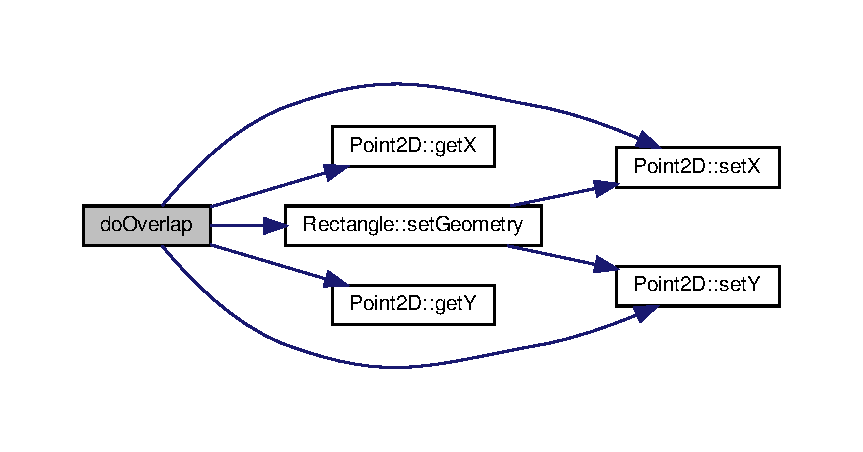
\includegraphics[width=350pt]{main_8cpp_a888d2b0113947b4461107bb02b28799d_cgraph}
\end{center}
\end{figure}
\mbox{\Hypertarget{main_8cpp_a5fe7cf71c1f13eed4b8144d0e00dc58d}\label{main_8cpp_a5fe7cf71c1f13eed4b8144d0e00dc58d}} 
\index{main.\+cpp@{main.\+cpp}!is\+Inside@{is\+Inside}}
\index{is\+Inside@{is\+Inside}!main.\+cpp@{main.\+cpp}}
\subsubsection{\texorpdfstring{is\+Inside()}{isInside()}}
{\footnotesize\ttfamily bool is\+Inside (\begin{DoxyParamCaption}\item[{const \hyperlink{classPoint2D}{Point2D} \&}]{p,  }\item[{const \hyperlink{classRectangle}{Rectangle} \&}]{r }\end{DoxyParamCaption})}



Calculates whether a point is internal to a rectangle. 


\begin{DoxyParams}{Parameters}
{\em p} & The point \\
\hline
{\em r} & The rectangle \\
\hline
\end{DoxyParams}
\begin{DoxyReturn}{Returns}

\end{DoxyReturn}

\begin{DoxyRetVals}{Return values}
{\em true} & if {\ttfamily p} is inscribed within {\ttfamily r}, \\
\hline
{\em false} & otherwise \\
\hline
\end{DoxyRetVals}


Definition at line 221 of file main.\+cpp.


\begin{DoxyCode}
221                                                     \{
222     \textcolor{keywordflow}{return} r.\hyperlink{classRectangle_a812afd6deed0cdec0b4ad7b2bd93871d}{getTopLeft}().\hyperlink{classPoint2D_a5cb1c2584e5b2bada0226a3e32aa2b1a}{getX}() <= p.\hyperlink{classPoint2D_a5cb1c2584e5b2bada0226a3e32aa2b1a}{getX}() && p.\hyperlink{classPoint2D_a5cb1c2584e5b2bada0226a3e32aa2b1a}{getX}()<=r.
      \hyperlink{classRectangle_a5f30a92f3fc197dda50d9e59995d3ac1}{getBottomRight}().\hyperlink{classPoint2D_a5cb1c2584e5b2bada0226a3e32aa2b1a}{getX}() &&
223            r.\hyperlink{classRectangle_a812afd6deed0cdec0b4ad7b2bd93871d}{getTopLeft}().\hyperlink{classPoint2D_a53d10f2e460c47a493a3fbadfbafbb64}{getY}() >= p.\hyperlink{classPoint2D_a53d10f2e460c47a493a3fbadfbafbb64}{getY}() && p.\hyperlink{classPoint2D_a53d10f2e460c47a493a3fbadfbafbb64}{getY}()>=r.
      \hyperlink{classRectangle_a5f30a92f3fc197dda50d9e59995d3ac1}{getBottomRight}().\hyperlink{classPoint2D_a53d10f2e460c47a493a3fbadfbafbb64}{getY}(); 
224 \}
\end{DoxyCode}
Here is the call graph for this function\+:
\nopagebreak
\begin{figure}[H]
\begin{center}
\leavevmode
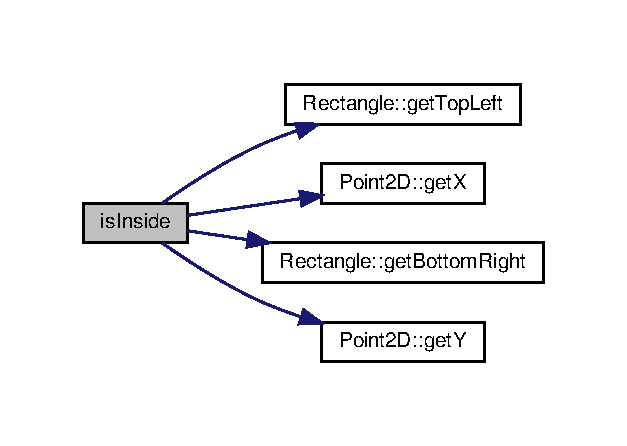
\includegraphics[width=301pt]{main_8cpp_a5fe7cf71c1f13eed4b8144d0e00dc58d_cgraph}
\end{center}
\end{figure}
\mbox{\Hypertarget{main_8cpp_ae66f6b31b5ad750f1fe042a706a4e3d4}\label{main_8cpp_ae66f6b31b5ad750f1fe042a706a4e3d4}} 
\index{main.\+cpp@{main.\+cpp}!main@{main}}
\index{main@{main}!main.\+cpp@{main.\+cpp}}
\subsubsection{\texorpdfstring{main()}{main()}}
{\footnotesize\ttfamily int main (\begin{DoxyParamCaption}{ }\end{DoxyParamCaption})}



Main function. 

\begin{DoxyReturn}{Returns}
Always 0 
\end{DoxyReturn}


Definition at line 230 of file main.\+cpp.


\begin{DoxyCode}
230            \{
231     \hyperlink{classRectangle}{Rectangle} A, B, Intersection;
232     \hyperlink{classPoint2D}{Point2D} p; 
233     \textcolor{keywordtype}{int} count;
234     
235     A.\hyperlink{classRectangle_a31c4b9fc0d1ddf912f114da494e50205}{setGeometry}(2,5,3,3);
236     cout << \textcolor{stringliteral}{"First rectangle is "}; 
237     A.\hyperlink{classRectangle_a4e315c59754599c74e99e8b31f7031a0}{print}();
238     cout << endl << \textcolor{stringliteral}{"Type second rectangle: "};
239     B.\hyperlink{classRectangle_af6973ed3094f9dbabeadb071772fa76d}{read}();
240     cout << endl << \textcolor{stringliteral}{"Calculating intersection of: "};
241     A.\hyperlink{classRectangle_a4e315c59754599c74e99e8b31f7031a0}{print}();
242     cout << \textcolor{stringliteral}{" and "};
243     B.\hyperlink{classRectangle_a4e315c59754599c74e99e8b31f7031a0}{print}();
244     cout << endl;
245     Intersection = \hyperlink{main_8cpp_a888d2b0113947b4461107bb02b28799d}{doOverlap}(A,B);
246     \textcolor{keywordflow}{if} (Intersection.\hyperlink{classRectangle_af732bce8c96d2469994825e9a87dbe5f}{isEmpty}()) \{
247         cerr << \textcolor{stringliteral}{"Empty intersection"}<<endl;
248     \} \textcolor{keywordflow}{else} \{
249         cout << \textcolor{stringliteral}{"The intersection is: "};
250         Intersection.\hyperlink{classRectangle_a4e315c59754599c74e99e8b31f7031a0}{print}();
251         count = 0;
252         cout << endl << \textcolor{stringliteral}{"Reading points..."};
253         p.\hyperlink{classPoint2D_ac13d12003e2da9afee19a6a3f526c660}{read}();
254         \textcolor{keywordflow}{while} (p.\hyperlink{classPoint2D_a5cb1c2584e5b2bada0226a3e32aa2b1a}{getX}()>=0 && p.\hyperlink{classPoint2D_a53d10f2e460c47a493a3fbadfbafbb64}{getY}()>=0) \{
255             \textcolor{keywordflow}{if} (\hyperlink{main_8cpp_a5fe7cf71c1f13eed4b8144d0e00dc58d}{isInside}(p,Intersection)) \{
256                 p.\hyperlink{classPoint2D_a4be0cc5bb62eef12bfa55ced97d03535}{print}();
257                 count ++;
258             \} 
259             p.\hyperlink{classPoint2D_ac13d12003e2da9afee19a6a3f526c660}{read}();
260         \}
261         \textcolor{keywordflow}{if} (count > 0)
262             cout << \textcolor{stringliteral}{" fall within the intersection ("}<< count<<\textcolor{stringliteral}{" total)"} << endl;
263         \textcolor{keywordflow}{else}
264             cout << \textcolor{stringliteral}{" None of them falls within the intersection "}<<endl;
265     \}
266 
267     \textcolor{keywordflow}{return} 0;
268 \}
\end{DoxyCode}
Here is the call graph for this function\+:
\nopagebreak
\begin{figure}[H]
\begin{center}
\leavevmode
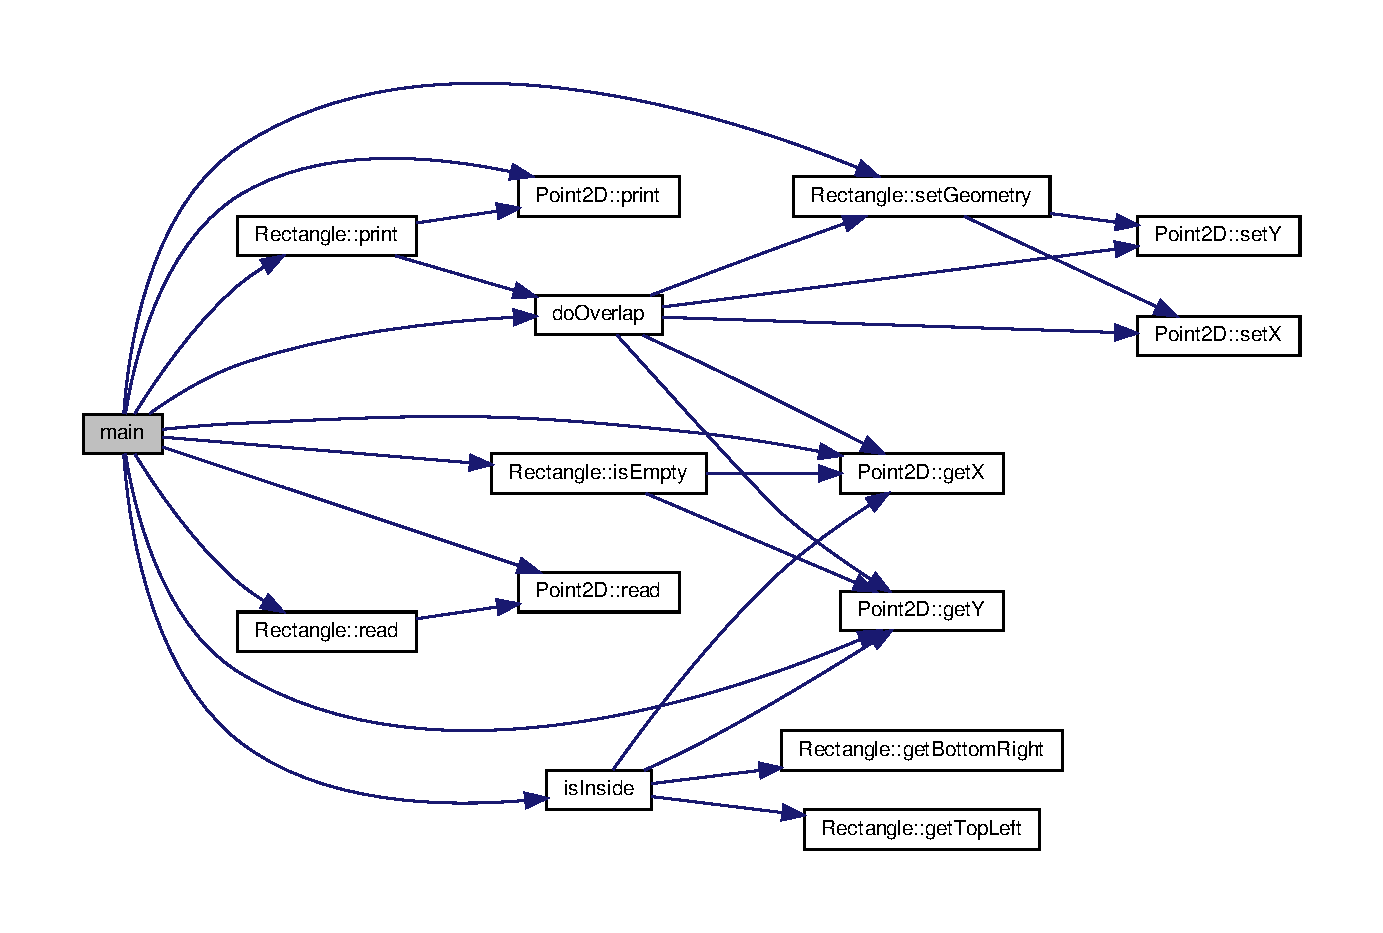
\includegraphics[width=350pt]{main_8cpp_ae66f6b31b5ad750f1fe042a706a4e3d4_cgraph}
\end{center}
\end{figure}

%--- End generated contents ---

% Index
\backmatter
\newpage
\phantomsection
\clearemptydoublepage
\addcontentsline{toc}{chapter}{Index}
\printindex

\end{document}
